\subsection{Discussion}
\subsubsection{Computational Performance of EKF-SLAM}
EKF-SLAM has been criticised for a variety of reasons in the literature, and one of the issues often brought up is computational performance as the map grows. Keeping the computation time down is of paramount importance in the online SLAM problem where delayed updates are not acceptable. In fact, each timestep of EKF-SLAM has a computational complexity of $\mathcal{O}(n^2)$ in the number of detected landmarks\cite{divideandconq}, something our implementation confirms. When tuned to provoke lots of landmark detections (around 800), the update step of the Kalman filter takes quadratic time, as shown in figure \ref{fig:a3-update_time_landmarks}. These results show that in large environments, EKF-SLAM alone fails to meet the time-requirements for online SLAM.

\begin{figure}
    \centering
    \begin{subfigure}{0.45\textwidth}
        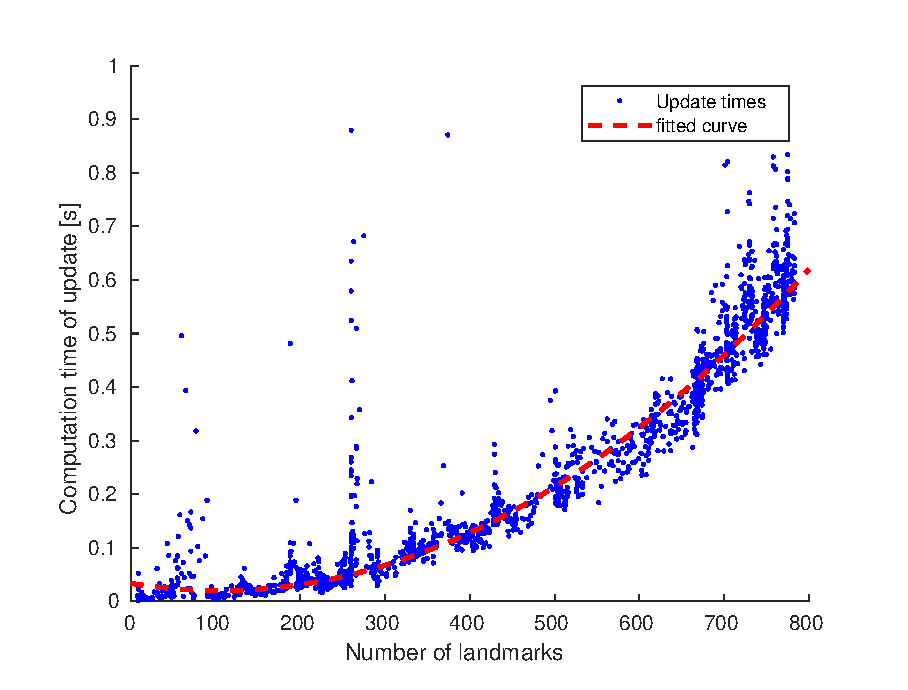
\includegraphics[width=\textwidth]{plots/a3/update-time-vs-landmarks}
        \caption{Update time vs landmarks}
        \label{fig:a3-update_time_landmarks}
    \end{subfigure}
    \begin{subfigure}{0.45\textwidth}
        \includegraphics[width=\textwidth]{plots/a3-real-results-bg}
        \caption{Trajectory overlayed Google Maps}
        \label{fig:a3-real-results_bg}
    \end{subfigure}
    \begin{subfigure}{0.45\textwidth}
        \includegraphics[width=\textwidth]{plots/a3-real-nis}
        \caption{NIS}
        \label{fig:a3-real-nis}
    \end{subfigure}
    \begin{subfigure}{0.45\textwidth}
        \includegraphics[width=\textwidth]{plots/a3-real-gnss-diff}
        \caption{SLAM vs GNSS}
        \label{fig:a3-real-gnss-diff}
    \end{subfigure}

    \caption{Victoria Park results}
\end{figure}
\subsubsection{Measurement Clutter}
After a successful run of the EKF-SLAM algorithm on the Victoria Park dataset, we typically find around  landmarks. For this reason, we have speculated that not all these landmarks correspond to actual trees, even though that is what they are supposed to represent. One of the reasons for this is landmarks being doubly registered due to the JCBB algorithm not making the proper associations. But another reason that must not be overlooked is the effect of clutter in the measurement data. The laser data in the dataset has been processed to only contain measurements that match a certain tree-profile\cite{victoria}, however, no classification algorithm is perfect and we speculate that a lot of the measurements are spurious and should be regarded as clutter. This partly stems from the fact that a lot of the detected landmarks happen to appear inside the six-lane intersection to the east of Victoria Park, as can be seen in figure \ref{fig:results_bg}. In our experiments, the effect of clutter has not been significant, and spuriously detected landmarks have not had a noticeable impact on SLAM performance. It might however become problematic for longer operation times and larger maps. Keeping the number of landmarks down is essential to successfully apply EKF-SLAM in an online situation. In addition, wrongly registered landmarks might lead to spurious associations in the future and ultimately worsen the tracking performance. In our implementation, all unassociated measurements are initialized as new landmarks and never face the possibility of removal, there are however techniques to remove landmarks which have low probability of corresponding to an actual real life feature. One possibility would be to employ something akin to the IPDA mentioned in \ref{sec:a1} since it has a concept of target existance that in a SLAM context could be used to discriminate false landmarks.

\subsubsection{Choice of JCBB CI Bounds and Implication for Robustness}
The JCBB algorithm operates with two confidence intervals, one for joint and one for individual compatibility. The Mahalonobis distances of both joint and individual compatibility are gated with these confidence intervals to determine whether to move on with a given hypothesis.\cite{jcbb} This is very similar to the measurement gating used for the IMM-PDAF in assignment 1. Similar to \cref{sec:imm-pdaf-gate-size} the confidence intervals are given by the $\chi^2$ distribution using $\alpha_1$ and $\alpha_2$ as significance. In the Victoria Park dataset, we found that the choice of large confidence intervals ($\alpha_1 = 10^{-5}$ and $\alpha_2 = 10^{-3}$ for joint and individual respectively) gave perfectly satisfactory association speed on the dataset, however when EKF-SLAM was rerun on the generated map with a slight offset in orientation of $6^\circ$ (such a situation could appear naturally from disturbances such temporary loss of sensor data), the JCBB algorithm wound up in an almost complete stall after a few hundred timesteps, likely because the offset pushed the likeliness of all the hypotheses closer together, making the algorithm unable to reduce the search tree and single out the best association in reasonable time. Choosing tighter confidence intervals on the other hand, with $\alpha = 0.1$ for both joint and individual, caused the EKF to lose track on many occasions, likely because the JCBB gated out important correct associations. With $\alpha = 0.001$ instead however, only the most promising hypotheses were considered, ultimately leading to reasonable execution times. We suppose then that one must be careful in choosing these variables and find a good tradeoff between speed and accuracy. In the end, these values made the rerun on the previously built map perfectly possible with no significant slow-down. This result shows how the choice of these confidence intervals is detrimental to the robustness of EKF-SLAM and crucial for online SLAM as a small disturbance can cause the JCBB algorithm to fail to find associations within reasonable time.

